\documentclass[11pt,a4paper]{article}

\usepackage[margin=2.3cm]{geometry}
\usepackage[T1]{fontenc}
\usepackage[utf8]{inputenc}
\usepackage{lmodern}
\usepackage{amsmath,amssymb,amsthm}
\usepackage{graphicx}
\usepackage{booktabs}
\usepackage{array}
\usepackage{caption}
\usepackage{xcolor}
\usepackage[hidelinks]{hyperref}

\graphicspath{{../data/medidrone/}{../results/}}

\newtheorem{theorem}{Theorem}
\newtheorem{proposition}[theorem]{Proposition}
\newtheorem{lemma}[theorem]{Lemma}
\theoremstyle{definition}
\newtheorem{definition}[theorem]{Definition}
\theoremstyle{remark}
\newtheorem{remark}[theorem]{Remark}

\newcommand{\code}[1]{\texttt{#1}}
\newcommand{\Ocal}{\mathcal{O}}

\title{CMP 3005 Term Project\\[2pt]
\large MediDrone Capacitated Vehicle Routing Problem (CVRP)}
\author{Team Student IDs: 2366912, 2364460\\
Official seed: $11372 = 6912 + 4460$}
\date{}

\begin{document}
\maketitle

\begin{abstract}
We model drone delivery of medical supplies across Istanbul as a Capacitated Vehicle
Routing Problem with a Bosphorus crossing penalty. We show that the decision version is
NP-complete, and we analyse how the penalty and the integer-rounded EUC\_2D distances
affect the triangle inequality. We implement three methods from scratch in Python:
a deterministic Clarke--Wright savings baseline, a memetic giant-tour genetic algorithm
with the Split decoder, and a route-based Tabu Search. We also implement an exact dynamic
program for instances with $n \le 12$. Every reported solution is validated by an
independent feasibility checker. Under an equal budget of 5\,s per run over 10 seeds,
the memetic GA reaches the best-known solution on A-n32-k5, achieves mean gaps of
2.29--8.53\% on the larger CVRPLIB A-instances, and returns cost 18548 on every seed for
\code{medidrone-n100-s11372}. Measured scaling exponents agree with the stated
asymptotic bounds.
\end{abstract}

% =====================================================================
\section{Problem Formulation and MediDrone Model}

\subsection{CVRP}
Let $G=(V,A)$ be a complete directed graph with $V=\{0,1,\dots,n\}$. Node $0$ is the depot,
and nodes $1,\dots,n$ are customers with integer demands $q_i \in [1,Q]$. A homogeneous
fleet of at most $K$ vehicles of capacity $Q$ starts and ends at the depot. Arc $(i,j)$ has
cost $c_{ij}$. A \emph{solution} is a set of routes $R_1,\dots,R_m$ with $m \le K$. Each route
is a sequence of customers, and the depot at the start and end is implicit, as in
\code{src/solution.py}. A solution is feasible when the following hold.
\begin{align}
&\textstyle\bigcup_{k=1}^{m} R_k = \{1,\dots,n\},\quad R_k \cap R_l = \emptyset\ (k\ne l)
&&\text{(each customer exactly once)}\\
&\textstyle\sum_{i\in R_k} q_i \le Q \quad \forall k &&\text{(capacity)}\\
&m \le K &&\text{(fleet bound)}
\end{align}
The objective is to minimise
\begin{equation}
\textstyle C(R_1,\dots,R_m) = \sum_{k=1}^{m}\Big( c_{0,r_{k,1}} + \sum_{t=1}^{|R_k|-1} c_{r_{k,t},\,r_{k,t+1}} + c_{r_{k,|R_k|},0}\Big).
\end{equation}
The cost matrix is $c_{ij} = d_{ij} + P\cdot[\sigma(i)\neq\sigma(j)]$, where
$d_{ij} = \lfloor \sqrt{(x_i-x_j)^2+(y_i-y_j)^2} + 0.5\rfloor$ is the TSPLIB EUC\_2D distance,
$\sigma(i)\in\{\mathrm{EU},\mathrm{AS}\}$ is the side of node $i$, and $P$ is the Bosphorus
penalty. CVRPLIB instances have no sides, which is equivalent to $P=0$.

\subsection{MediDrone Istanbul model}
\code{generate\_medidrone} in \code{src/parser\_generator.py} builds instances as follows.
\begin{itemize}
\item The service area is $[0,1000]^2$ with integer coordinates, and the depot is at $(500,500)$.
\item The Bosphorus is the line $x=500$. A node is on the European side if $x<500$ and on the
  Asian side if $x\ge 500$. The depot is therefore on the Asian side.
\item Customer locations: the generator draws 4--6 cluster centres, alternating Europe
  ($x\in[100,450]$) and Asia ($x\in[550,900]$), with $y\in[100,900]$. It places 80\% of the
  customers round-robin around the centres using a Gaussian with $\sigma=50$, clipped to
  the square. The remaining 20\% are uniform over the square.
\item Demand $q_i \sim \mathcal{U}\{1,\dots,30\}$, $Q=100$, $K=\lceil \sum_i q_i / Q\rceil + 1$.
\item Every arc between the two sides costs an extra $P=150$.
\end{itemize}
With the team seed $11372$ the generator draws 5 clusters. The instance
\code{medidrone-n100-s11372} has $n=100$, $\sum_i q_i = 1575$, $Q=100$ and $K=17$. Of its
customers, 60 are in Europe and 40 in Asia (Figure~\ref{fig:medidrone}).

\begin{figure}[ht]
\centering
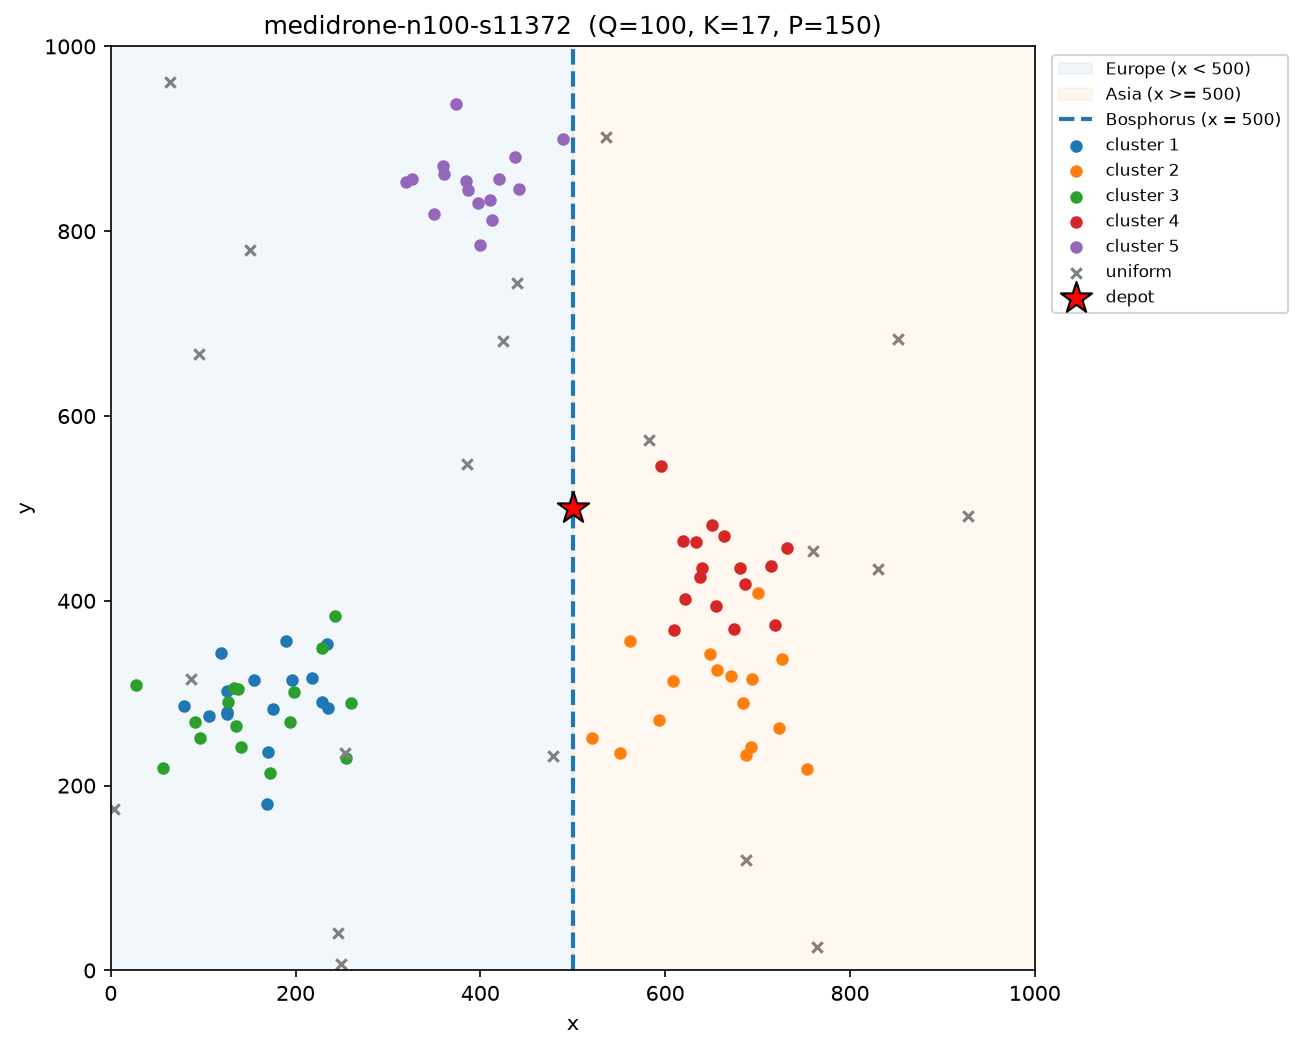
\includegraphics[width=0.62\linewidth]{medidrone-n100-s11372.png}
\caption{The \code{medidrone-n100-s11372} instance ($n=100$, $\sum q_i=1575$, $Q=100$, $K=17$).
Colours mark the five generated clusters, and grey points are uniform customers. The
vertical line $x=500$ is the Bosphorus, and every arc that crosses it costs an extra
$P=150$. The depot is at $(500,500)$, on the Asian side.}
\label{fig:medidrone}
\end{figure}

% =====================================================================
\section{Computational Complexity and Theoretical Analysis}

\begin{definition}[CVRP-D]
Given an instance $I=(n, (c_{ij}), (q_i), Q, K)$ with integer data and an integer bound $B$,
is there a feasible solution with $C \le B$?
\end{definition}

\begin{theorem}
CVRP-D $\in$ NP.
\end{theorem}
\begin{proof}
\emph{Certificate.} A list of at most $K$ routes, each a list of customer ids. A valid
certificate contains exactly $n$ customer entries and at most $K$ route separators, so its
size is $\Ocal(n+K)$, which is polynomial in the input size.

\emph{Verifier.} The verifier follows \code{check\_solution} in \code{src/feasibility.py},
which runs five checks in sequence:
\begin{enumerate}
\item \code{check\_indices}: every entry is an integer in $[1,n]$.
\item \code{check\_coverage}: a count array of length $n$ shows that each customer appears exactly once.
\item \code{check\_capacity}: for each route, the sum of its demands is at most $Q$.
\item \code{check\_fleet}: the number of non-empty routes is at most $K$.
\item \code{recompute\_cost}: the cost is summed over the arcs $0\to r_1\to\dots\to r_\ell\to 0$
  of every route, and the result is compared with $B$.
\end{enumerate}
Checks 1--3 and 5 read each entry a constant number of times. Check 4 and the depot arcs
in check 5 add $\Ocal(1)$ work per route. Each arc cost is $\Ocal(1)$: either a matrix
lookup, or the EUC\_2D formula plus one side comparison. The verifier therefore runs in
$\Ocal(n+K)$ time once the instance is read. A certificate longer than $n+K$ entries is
rejected after reading $\Ocal(n+K)$ of it.
\end{proof}

\begin{theorem}
CVRP-D is NP-hard, even for Euclidean instances with $P=0$. Hence CVRP-D is NP-complete.
\end{theorem}
\begin{proof}
We reduce from the decision version of Euclidean TSP: given points $p_0,\dots,p_n$ with
integer coordinates and a bound $B$, is there a Hamiltonian cycle of rounded EUC\_2D
length at most $B$? This problem is NP-complete~\cite{papadimitriou1977,garey1976}.

\emph{Construction.} Make $p_0$ the depot and $p_1,\dots,p_n$ the customers. Set
$q_i=1$ for all $i$, $Q=n$ (any $Q\ge\sum_i q_i$ works), $K=1$, $P=0$ (no sides), and keep
$B$. The construction takes $\Ocal(n)$ time, or $\Ocal(n^2)$ if the cost matrix is written
out explicitly.

\emph{Correctness.} With $K=1$, a feasible CVRP solution is exactly one route that visits
every customer once, starting and ending at the depot. That route is a Hamiltonian cycle
on $\{p_0,\dots,p_n\}$, and its CVRP cost equals the tour length because $P=0$. The capacity
constraint $\sum q_i = n \le Q$ always holds. So a CVRP solution of cost at most $B$ exists
if and only if a TSP tour of length at most $B$ exists. Combined with Theorem~1, CVRP-D is
NP-complete.
\end{proof}

\subsection{The Bosphorus penalty and the triangle inequality}
The penalty is a function of the two endpoint \emph{sides}. It does not depend on whether
the straight segment between the endpoints crosses $x=500$. This makes the penalty a cut
semimetric.

\begin{proposition}\label{prop:metric}
Let $\bar c_{ij} = e_{ij} + P\,\delta_{ij}$, where $e_{ij}$ is the exact (unrounded)
Euclidean distance and $\delta_{ij}=[\sigma(i)\ne\sigma(j)]$. For every $P\ge0$, $\bar c$
satisfies $\bar c_{uv} \le \bar c_{uw} + \bar c_{wv}$ for all $u,v,w$.
\end{proposition}
\begin{proof}
$e$ satisfies the triangle inequality. For $\delta$, check the two cases.
If $\sigma(u)=\sigma(v)$, then $\delta_{uv}=0\le\delta_{uw}+\delta_{wv}$.
If $\sigma(u)\ne\sigma(v)$, then $w$ differs from at least one of $u$ and $v$, so
$\delta_{uw}+\delta_{wv}=1 = \delta_{uv}$. The sum of two functions that satisfy the
triangle inequality also satisfies it, with $P\ge 0$ as the weight on $\delta$.
\end{proof}

The two cases in the proof cover the two situations from the problem statement.
\begin{itemize}
\item \emph{Same-side detour across the Bosphorus.} Let $u,v\in\mathrm{EU}$ and
  $w\in\mathrm{AS}$. The detour $u\to w\to v$ pays $2P=300$, while the direct arc pays
  nothing, so the detour never shortcuts the direct arc.
\item \emph{Cross-side.} Let $u\in\mathrm{EU}$ and $v\in\mathrm{AS}$. Every path from $u$
  to $v$ crosses an odd number of times, so it pays at least $P$, the same as the direct arc.
\end{itemize}
The side-based penalty with $P=150$ therefore does \emph{not} by itself break the triangle
inequality. Any violation in the implemented cost matrix comes from the nearest-integer
rounding of $d$. Rounding changes each distance by at most $\tfrac12$:
\[
c_{uv} \le e_{uv} + \tfrac12 + P\delta_{uv} \le \bar c_{uw} + \bar c_{wv} + \tfrac12
\le c_{uw} + c_{wv} + \tfrac32 .
\]
Since all costs are integers, $c_{uv} \le c_{uw}+c_{wv}+1$, so the violation is at most one
unit. The following counterexamples were computed with the project's own
\code{ProblemInstance.cost} ($P=150$).
\begin{itemize}
\item \emph{Same side.} $u=(0,0)$, $w=(1,1)$, $v=(2,2)$, all in EU:
  $c_{uw}=c_{wv}=\lfloor 1.414+0.5\rfloor = 1$, but $c_{uv}=\lfloor 2.828+0.5\rfloor = 3 > 2$.
\item \emph{Cross side, via the depot.} $u=(498,498)\in\mathrm{EU}$, $w=(499,499)\in\mathrm{EU}$,
  $v=(500,500)$, the depot, in AS: $c_{uw}=1$, $c_{wv}=1+150=151$, but
  $c_{uv}=3+150=153 > 152$.
\end{itemize}

\begin{remark}
In both counterexamples the violation is one unit and does not depend on $P$. The penalty
matters for the structure of solutions rather than for metricity. The depot is in Asia, so
every route that serves at least one European customer crosses at least twice. Its cost
therefore includes at least $2P=300$. In Clarke--Wright, the saving of two European
customers $i,j$ is $s_{ij} = c_{i0}+c_{0j}-c_{ij}$. Both $c_{i0}$ and $c_{0j}$ include $P$,
so $s_{ij}$ grows by $2P$, and the algorithm merges European customers early.
\end{remark}

% =====================================================================
\section{Algorithms, Implementation and Asymptotic Complexity}
All algorithms use the same cost matrix (\code{inst.cost}, penalty included). They are
written in plain Python without any VRP or metaheuristic library. Throughout, $L$ denotes
the maximum number of customers on a route.

\subsection{Clarke--Wright savings baseline (\code{src/clarke\_wright.py})}
The baseline is the parallel savings algorithm~\cite{clarke1964}.
\begin{enumerate}
\item Start with one route per customer.
\item Compute $s_{ij}=c_{i0}+c_{0j}-c_{ij}$ for all pairs $i<j$, and sort the savings in
  decreasing order.
\item Scan the sorted list. Merge the routes of $i$ and $j$ when the routes are different,
  $i$ and $j$ are both route endpoints, and the combined load is at most $Q$. Reversing a
  route is allowed, since costs are symmetric.
\item Stop at the first non-positive saving, unless the solution still has more than $K$
  routes. In that case, non-positive merges continue in order to reduce the fleet.
\item If more than $K$ routes remain, \code{repair\_fleet} empties the smallest route. It
  moves each customer to its cheapest capacity-feasible insertion position in another
  route. It stops cleanly if some customer fits nowhere, and \code{feasibility.py} then
  reports the fleet violation.
\end{enumerate}
\emph{Complexity.} Computing the savings costs $\Ocal(n^2)$ and sorting them costs
$\Ocal(n^2\log n)$. Each candidate pair is checked in $\Ocal(1)$. There are at most $n-1$
merges, each costing $\Ocal(n)$ to relabel route ids. The total is
$\Ocal(n^2\log n)$ time and $\Ocal(n^2)$ space for the savings list. Removing one route in
the repair costs $\Ocal(n^2)$, and $\Ocal(n^3)$ in the worst case if $\Ocal(n)$ routes had to
be removed. The algorithm is deterministic, so it is run once per instance.

\subsection{Memetic giant-tour GA with the Split decoder (\code{src/ga\_split.py})}
\paragraph{Representation.} A chromosome is a permutation of $1..n$, called a giant tour,
with no depot visits. The Split decoder~\cite{prins2004} determines the route boundaries
optimally for a given order.

\paragraph{Split.} Build a DAG on nodes $0..m$. Arc $(i,j)$ represents the route
$t_i,\dots,t_{j-1}$ and exists only if that route's load is at most $Q$. Its weight is
$w(i,j) = c_{0t_i} + \sum_{k=i}^{j-2} c_{t_kt_{k+1}} + c_{t_{j-1}0}$. Bellman's recursion
\[
V_0 = 0, \qquad V_j = \min_{i<j,\;(i,j)\text{ exists}} V_i + w(i,j)
\]
gives the optimal split. Each weight is extended in $\Ocal(1)$ from the previous one, and
the inner loop stops as soon as the load exceeds $Q$. Split is therefore $\Ocal(nL)$ when
capacity is binding and $\Ocal(n^2)$ when it is not ($Q\ge\sum q_i$).

\paragraph{Fleet bound.} If the unbounded Split uses more than $K$ routes,
\code{split\_bounded} runs the same DP with a route-count dimension in $\Ocal(KnL)$.
\code{min\_routes} fills routes greedily along the order, which gives the fewest routes any
split of that order can use. The fitness is the pair
$(\text{routes over }K,\ \text{cost})$, compared lexicographically. Any fleet-feasible order
beats any infeasible one, and no penalty weight has to be tuned.

\paragraph{Operators and parameters.}
\begin{itemize}
\item \emph{Population:} 50 individuals. The initial population is the Clarke--Wright giant
  tour plus random permutations.
\item \emph{Selection and crossover:} binary tournament selection, then Order Crossover (OX).
\item \emph{Mutation:} with probability $p_m=0.2$, either a swap or a segment inversion,
  each with probability $\tfrac12$.
\item \emph{Elitism:} the 2 best individuals survive unchanged.
\item \emph{Local search:} every initial individual, and each child with probability 0.2,
  receives local search, which makes the GA memetic.
\end{itemize}
The local search alternates two moves until neither improves:
\begin{itemize}
\item first-improvement intra-route 2-opt, with $\Delta = c_{ac}+c_{bd}-c_{ab}-c_{cd}$;
\item granular inter-route relocate, restricted to the $G=10$ nearest neighbours, costing
  $\Ocal(nGL)$ per pass instead of $\Ocal(n^2)$.
\end{itemize}
Local search never raises the cost, never breaks capacity and never adds a route. The
improved routes are re-encoded as the child's giant tour. Each new best solution is
checked by \code{feasibility.py}.

\subsection{Route-based Tabu Search (\code{src/tabu\_search.py})}
\paragraph{Neighbourhood.} Each iteration evaluates three neighbourhoods in full:
\begin{itemize}
\item \emph{relocate:} move customer $u$ from route $A$ to any position in another route
  $B$, provided $\ell_B+q_u\le Q$. This may empty $A$.
\item \emph{inter-route swap:} exchange $u\in A$ with $v\in B$, provided both new loads are
  at most $Q$.
\item \emph{intra-route 2-opt:} reverse a segment of a route.
\end{itemize}
The search applies the best admissible move, even if it increases the cost.

\paragraph{$\Ocal(1)$ deltas.} Each move changes only the arcs adjacent to the touched
positions. Let $p$ be the route path with the depot at both ends.
\begin{itemize}
\item \emph{Relocate} of $u=p_i$ from $A$ to between $p'_{j-1}$ and $p'_j$ in $B$:
  $\Delta = c_{p_{i-1}p_{i+1}} - c_{p_{i-1}u} - c_{up_{i+1}} + c_{p'_{j-1}u} + c_{up'_j} - c_{p'_{j-1}p'_j}$.
\item \emph{Swap} removes two arcs and adds two arcs in each of the two routes.
\item \emph{2-opt} uses $\Delta = c_{ac}+c_{bd}-c_{ab}-c_{cd}$.
\end{itemize}
All terms are read from \code{inst.cost}, so a change in the number of Bosphorus crossings
is already part of $\Delta$ and needs no separate update. A unit test compares 500 random
deltas against full recomputation on the MediDrone instance.

\paragraph{Fleet handling.} The fitness is $(\max(0, m-K),\ C)$, compared lexicographically
as in the GA. The search has no route-opening move. A start with more than $K$ routes can
only reduce its route count, by a relocate that empties a route.

\paragraph{Tabu list and aspiration.} Relocate and swap make the attribute
$(\text{node}, u, A)$ tabu, which forbids $u$ from re-entering route $A$. 2-opt makes the
removed arcs $(\text{arc}, a, b)$ tabu. The tenure is drawn uniformly from $[7,15]$ for each
move. A tabu move is still admissible if its fitness is strictly better than the best found
so far (aspiration). Ties among equal candidates are broken by seeded reservoir sampling.

\paragraph{Start solutions.} Seed 1 starts from Clarke--Wright. For seeds $>1$, the start
is a seeded random permutation decoded by Split, or by \code{split\_bounded} when more than
$K$ routes would be used. If no order fits in $K$ routes, up to 20 shuffles are tried, and
the order with the smallest excess is kept. This start is checked by \code{feasibility.py},
which permits only a fleet excess.

\paragraph{Complexity per iteration.} The neighbourhood sizes are:
\begin{itemize}
\item relocate: $n(n+R)$ positions, where $R$ is the number of routes;
\item swap: at most $n^2/2$ pairs;
\item 2-opt: $\sum_r L_r^2/2 = \Ocal(nL)$.
\end{itemize}
Each candidate costs $\Ocal(1)$, so one iteration takes $\Ocal(n^2)$ time, plus $\Ocal(n)$ to
apply the chosen move.

\subsection{Exact verifier for tiny instances (\code{solve\_exact})}
For $n\le12$, \code{src/parser\_generator.py} computes provably optimal solutions by
dynamic programming in two steps.
\begin{enumerate}
\item \emph{Held--Karp:} compute the cheapest single route for every capacity-feasible
  customer subset. This takes $\Ocal(2^n n^2)$ time.
\item \emph{Set partitioning:} compute
  $f_r(M)=\min_{S\subseteq M,\ \min M\in S} \mathrm{route}(S) + f_{r-1}(M\setminus S)$, then
  take $\min_{r\le K} f_r(\{1..n\})$. Fixing the lowest customer of $M$ in $S$ removes
  symmetric duplicates. Enumerating submasks costs $\Ocal(K\,3^n)$.
\end{enumerate}
The tiny instances have $Q=20$. The optima, stored in \code{data/tiny/*.sol}, are 324 for
\code{tiny-n7-s1} ($K=3$), 440 for \code{tiny-n8-s2} ($K=4$) and 342 for
\code{tiny-n9-s3} ($K=4$). These values serve as ground truth for the heuristics.

% =====================================================================
\section{Experimental Setup}
\code{src/complexity\_experiments.py} runs every algorithm on three groups of instances:
\begin{itemize}
\item the three tiny instances;
\item the CVRPLIB set A instances A-n32-k5, A-n45-k6, A-n60-k9 and A-n80-k10, with best
  known solutions (BKS) 784, 944, 1354 and 1763 taken from their \code{.sol} files;
\item \code{medidrone-n100-s11372}.
\end{itemize}
Clarke--Wright is deterministic and runs once per instance. The GA and Tabu Search each
run with seeds $1,\dots,10$ and an equal wall-clock budget of 5\,s per run. Their
iteration caps are set high enough that only the time limit stops them.

Each run is checked by \code{check\_solution}, and the CSVs record \code{is\_valid} and the
error list. The cost statistics in the tables are computed over valid runs only, and
$\text{gap} = 100\,(C-\text{BKS})/\text{BKS}$. All numbers in Sections~\ref{sec:results}
and~\ref{sec:scaling} come from \code{results/summary.csv}, \code{results/runs.csv} and
\code{results/scaling.csv}.

% =====================================================================
\section{Results}\label{sec:results}

\subsection{Tiny instances against the exact optimum}
\begin{table}[ht]
\centering
\caption{Tiny instances (10 seeds for the GA and Tabu Search, 5\,s each). The optimum was
computed by \code{solve\_exact}.}
\label{tab:tiny}
\begin{tabular}{lrrrrrrr}
\toprule
Instance & $n$ & $K$ & Optimum & CW & GA mean & Tabu mean & Tabu worst\\
\midrule
tiny-n7-s1 & 7 & 3 & 324 & 324 & 324 & 324.0 & 324\\
tiny-n8-s2 & 8 & 4 & 440 & 440 & 440 & 440.0 & 440\\
tiny-n9-s3 & 9 & 4 & 342 & 342 & 342 & 350.4 & 426\\
\bottomrule
\end{tabular}
\end{table}
Clarke--Wright and the GA (on all 10 seeds) reach the optimum on all three instances
(Table~\ref{tab:tiny}). Tabu Search reaches it in 29 of 30 runs. On \code{tiny-n9-s3},
seed 8 stays at 426, which is 24.56\% above the optimum, with 3 routes. The optimal
solution uses 4 routes. Tabu Search has no route-opening move, so it cannot leave the 3-route
structure that its random start produced.

\subsection{CVRPLIB benchmarks}
\begin{table}[ht]
\centering
\caption{CVRPLIB set A, 10 seeds, 5\,s per run. Mean $\pm$ std and gaps are computed over
valid runs; ``Feas.'' is the fraction of valid runs.}
\label{tab:bench}
\setlength{\tabcolsep}{4.2pt}
\begin{tabular}{lr rr rrrr rrrr}
\toprule
& & \multicolumn{2}{c}{Clarke--Wright} & \multicolumn{4}{c}{Memetic GA} & \multicolumn{4}{c}{Tabu Search}\\
\cmidrule(lr){3-4}\cmidrule(lr){5-8}\cmidrule(lr){9-12}
Instance & BKS & Cost & Gap\% & Mean $\pm$ std & Best & Gap\% & Feas. & Mean $\pm$ std & Best & Gap\% & Feas.\\
\midrule
A-n32-k5  & 784  & 842  & 7.40 & 784.0 $\pm$ 0.0   & 784  & 0.00 & 1.0 & 850.1 $\pm$ 39.0  & 796  & 8.43  & 1.0\\
A-n45-k6  & 944  & 997$^{\dagger}$ & -- & 1024.5 $\pm$ 37.9 & 954  & 8.53 & 1.0 & 964.0 $\pm$ 0.0 & 964 & 2.12 & 0.1\\
A-n60-k9  & 1354 & 1408 & 3.99 & 1385.0 $\pm$ 14.4  & 1365 & 2.29 & 1.0 & 1484.7 $\pm$ 58.1 & 1394 & 9.65  & 1.0\\
A-n80-k10 & 1763 & 1840 & 4.37 & 1835.9 $\pm$ 4.7   & 1823 & 4.14 & 1.0 & 2014.3 $\pm$ 101.7 & 1832 & 14.25 & 1.0\\
\bottomrule
\multicolumn{12}{l}{\footnotesize $^{\dagger}$Infeasible: 7 routes for $K=6$; not counted in any statistic.}
\end{tabular}
\end{table}

\begin{figure}[ht]
\centering
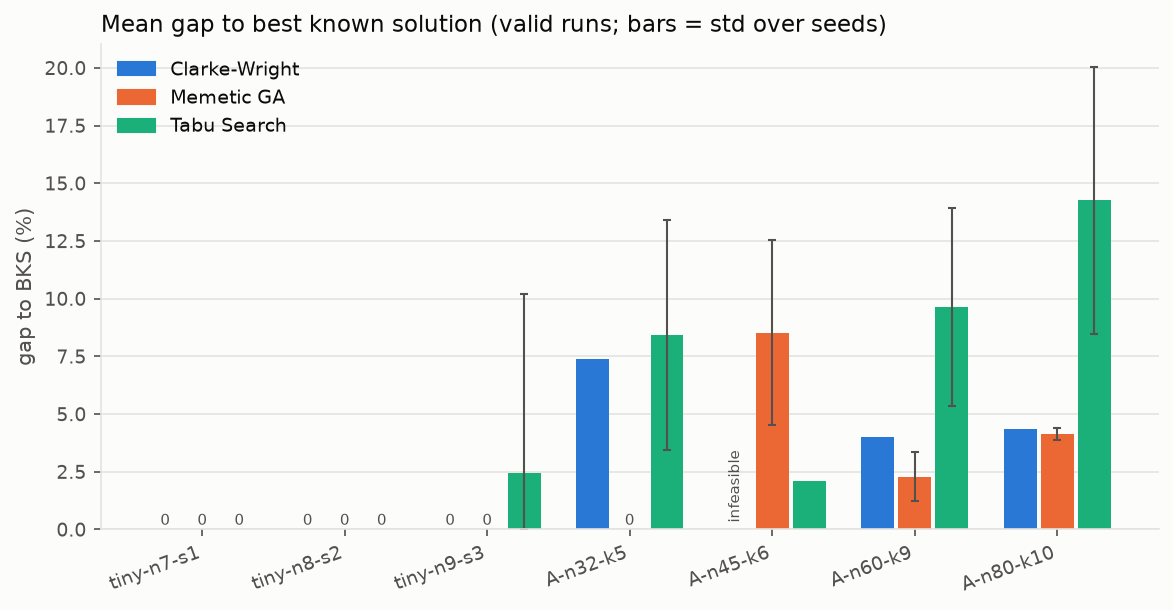
\includegraphics[width=0.85\linewidth]{gap_by_instance.png}
\caption{Mean gap to the best-known or optimal cost per instance and algorithm, over valid
runs (\code{results/gap\_by\_instance.png}).}
\label{fig:gaps}
\end{figure}

The memetic GA has the lowest mean gap on every benchmark. It reaches the BKS on
A-n32-k5 on all 10 seeds and is feasible in all 40 benchmark runs.

A-n45-k6 is the hardest case for fleet feasibility, with $\sum q_i = 593$ against a fleet
capacity of $6\cdot100=600$.
\begin{itemize}
\item \emph{Clarke--Wright} ends with 7 routes, and \code{repair\_fleet} cannot place the
  remaining customers into the spare capacity of the other routes.
\item \emph{Tabu Search} is feasible only for seed 1 (cost 964, 2.12\%), whose
  Clarke--Wright start the search reduces from 7 routes to 6. The other nine runs start from
  7-route random splits and remain at 7 routes (\code{runs.csv}).
\end{itemize}
On A-n60-k9 and A-n80-k10, Clarke--Wright beats the mean Tabu Search result. The best Tabu
runs (1394 and 1832) are close to the GA, but the spread across seeds is large (std 58.1 and
101.7). The random starts are weaker than the Clarke--Wright start, and 5\,s is not enough
for the search to recover from them.

\subsection{MediDrone instance}
\begin{table}[ht]
\centering
\caption{\code{medidrone-n100-s11372} ($K=17$, $P=150$), 10 seeds, 5\,s per run. All runs
are valid and use 17 routes.}
\label{tab:medidrone}
\begin{tabular}{lrrrrrr}
\toprule
Algorithm & Mean & Std & Best & Worst & Mean iterations & Mean runtime (s)\\
\midrule
Clarke--Wright & 18746 & --- & 18746 & 18746 & --- & 0.006\\
Memetic GA & 18548.0 & 0.0 & 18548 & 18548 & 27.0 generations & 5.089\\
Tabu Search & 19935.8 & 942.4 & 18479 & 21306 & 627.2 iterations & 5.083\\
\bottomrule
\end{tabular}
\end{table}

\begin{figure}[ht]
\centering
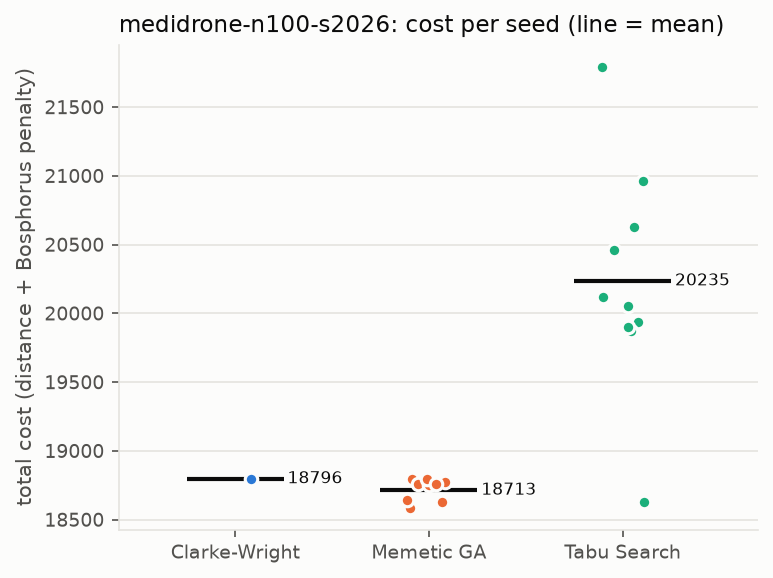
\includegraphics[width=0.7\linewidth]{medidrone_costs.png}
\caption{Per-seed costs on \code{medidrone-n100-s11372} (\code{results/medidrone\_costs.png}).}
\label{fig:medcosts}
\end{figure}

The GA returns 18548 on all 10 seeds, which is 1.06\% below Clarke--Wright
(Table~\ref{tab:medidrone}). The 5\,s budget allows a mean of 27 generations at $n=100$.
The Tabu Search results depend on the start:
\begin{itemize}
\item Seed 1 starts from Clarke--Wright and also ends at 18548.
\item Seed 6 starts from a random split and finds 18479, the lowest cost observed on this
  instance.
\item The remaining random-start runs end between 19365 and 21306.
\end{itemize}
No lower bound is available for this instance, so the costs are not reported as gaps.

% =====================================================================
\section{Empirical Scaling}\label{sec:scaling}
\code{measure\_scaling} times each step on MediDrone instances from the same generator,
with $n\in\{25,50,100,200,400\}$. Each time is the best of 3 repetitions, and the Tabu time
is the mean over 5 iterations. \code{split\_Q100} uses the instance capacity $Q=100$.
\code{split\_Qinf} sets $Q=\sum q_i$, so that a single route can carry everything. The
exponent $b$ is the slope of a least-squares fit of $\log t$ against $\log n$.

\begin{table}[ht]
\centering
\caption{Measured time per call in milliseconds (\code{results/scaling.csv}).}
\label{tab:scaling}
\begin{tabular}{lrrrrrcr}
\toprule
Step & $n=25$ & 50 & 100 & 200 & 400 & Theory & Fitted $b$\\
\midrule
Clarke--Wright run    & 0.287 & 1.167 & 5.038 & 21.941 & 125.378 & $\Ocal(n^2\log n)$ & 2.18\\
Split, $Q=100$        & 0.065 & 0.142 & 0.299 & 0.614  & 1.272   & $\Ocal(nL)$        & 1.07\\
Split, $Q=\infty$     & 0.144 & 0.553 & 2.160 & 8.609  & 38.503  & $\Ocal(n^2)$       & 2.01\\
Tabu iteration        & 0.737 & 1.966 & 9.613 & 32.327 & 111.918 & $\Ocal(n^2)$       & 1.85\\
\midrule
Mean route length $L$ & 4.17 & 4.55 & 4.55 & 4.76 & 4.60 & & \\
\bottomrule
\end{tabular}
\end{table}

\begin{figure}[ht]
\centering
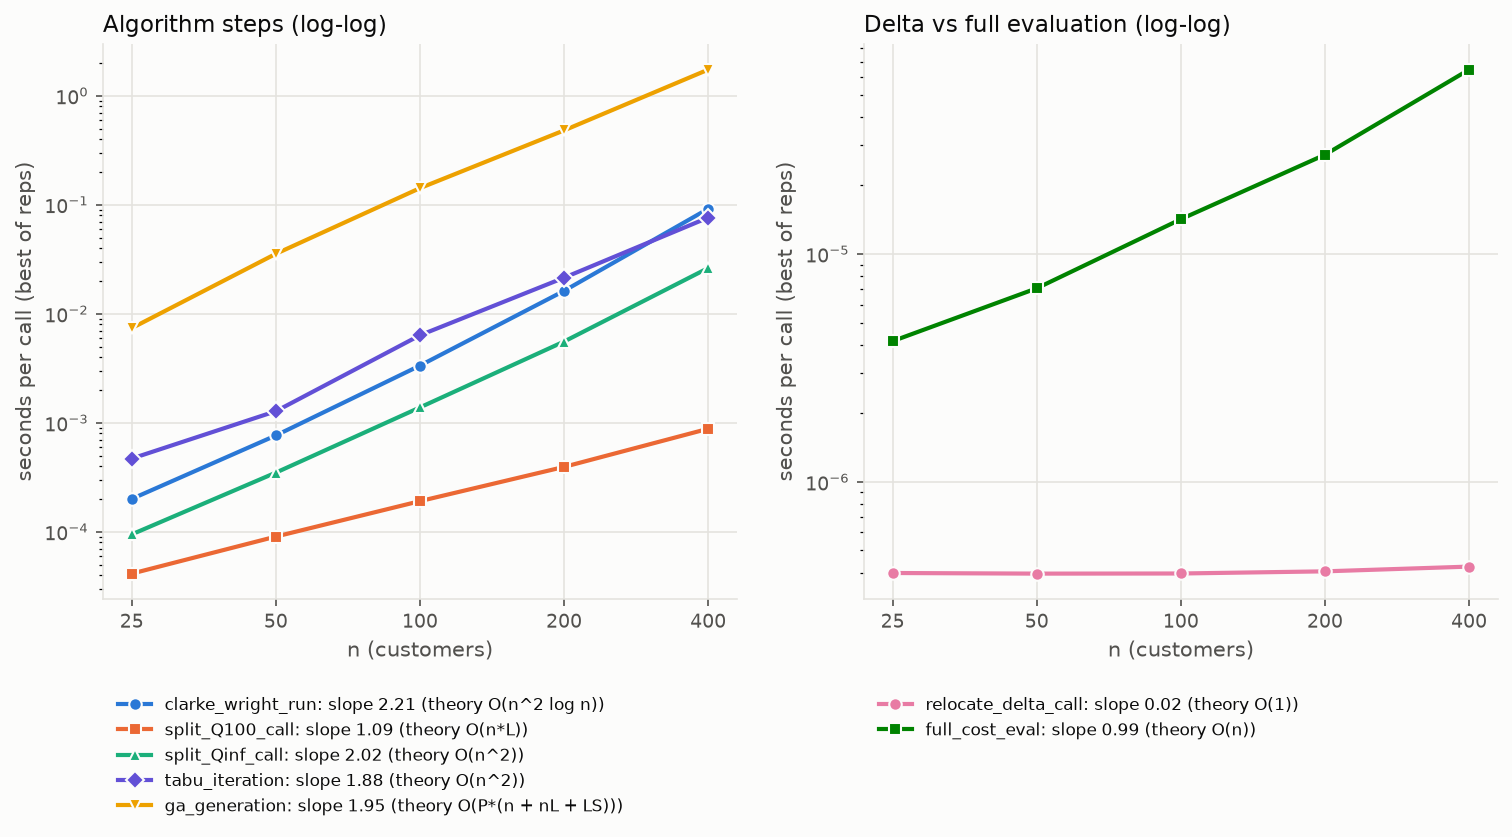
\includegraphics[width=0.8\linewidth]{scaling.png}
\caption{Log--log runtime against $n$ with fitted exponents (\code{results/scaling.png}).}
\label{fig:scaling}
\end{figure}

The fitted exponents match the analysis (Table~\ref{tab:scaling}).
\begin{itemize}
\item \emph{Split.} The mean route length stays between 4.17 and 4.76 as $n$ grows 16-fold,
  so the capacity-bounded Split grows linearly ($b=1.07$). The unbounded Split shows the
  quadratic worst case ($b=2.01$). At $n=400$ the gap between them is a factor of 30.
\item \emph{Clarke--Wright.} The exponent of 2.18 is above 2, consistent with the $\log n$
  factor from sorting the $\Theta(n^2)$ savings.
\item \emph{Tabu Search.} The exponent of 1.85 is slightly below 2. Part of each iteration
  scales linearly: the 2-opt neighbourhood is $\Ocal(nL)$ and applying a move is $\Ocal(n)$.
  At these sizes, these terms keep the measured slope below the $\Ocal(n^2)$ asymptote.
\end{itemize}

% =====================================================================
\section{Conclusion}
\begin{itemize}
\item \emph{Complexity.} CVRP-D is NP-complete, and the reduction from Euclidean TSP holds
  with $P=0$. The side-based Bosphorus penalty is a cut semimetric and preserves the
  triangle inequality. Only the EUC\_2D rounding violates it, by at most one unit.
\item \emph{Algorithms.} Under an equal 5\,s budget the memetic GA is the most reliable
  method. It is feasible in all runs, reaches the BKS on A-n32-k5, and has the lowest mean
  gap on every benchmark. Tabu Search produces individual runs that are competitive,
  including the best MediDrone cost of 18479. Its results depend heavily on the start
  solution, and without a route-opening move it cannot repair a fleet excess on tight
  instances such as A-n45-k6.
\item \emph{Scaling.} The measured exponents (2.18, 1.07, 2.01, 1.85) agree with the stated
  bounds.
\end{itemize}

% =====================================================================
\appendix
\section{Reproducibility}
All commands are run from the repository root with Python, numpy and matplotlib:
\begin{verbatim}
python -m src.parser_generator              # regenerate MediDrone + tiny instances
python -m src.complexity_experiments --time-limit 5 --seeds 10
python -m tests.test_feasibility            # likewise for the other test modules
\end{verbatim}

\section*{Appendix B: AI Tool Usage Statement}
\addcontentsline{toc}{section}{Appendix B: AI Tool Usage Statement}
% To be completed manually by the team.

\begin{thebibliography}{9}
\bibitem{papadimitriou1977}
C.~H. Papadimitriou, ``The Euclidean travelling salesman problem is NP-complete,''
\emph{Theoretical Computer Science}, 4(3):237--244, 1977.
\bibitem{garey1976}
M.~R. Garey, R.~L. Graham, D.~S. Johnson, ``Some NP-complete geometric problems,''
\emph{Proc. 8th ACM STOC}, 10--22, 1976.
\bibitem{prins2004}
C.~Prins, ``A simple and effective evolutionary algorithm for the vehicle routing problem,''
\emph{Computers \& Operations Research}, 31(12):1985--2002, 2004.
\bibitem{clarke1964}
G.~Clarke, J.~W. Wright, ``Scheduling of vehicles from a central depot to a number of
delivery points,'' \emph{Operations Research}, 12(4):568--581, 1964.
\end{thebibliography}

\end{document}
